\section{Optimal Policy under Conditional Independence}
Equation \eqref{eq:t1} can be written
\begin{equation}
	\begin{split}
		p(N_t^* > 0 | D, I) &= \sum_{s_1,\dots s_t}1_{N_{t}> 0}p(s_1,\dots s_t|D,I)\sum_{s_{t+1},\dots s_T}p(s_{t+1},\dots s_T|s_1,\dots s_t,D,I)\\
		& = \sum_{\zeta_t=0}^{N_0+\upsilon_t}p(\zeta_t|D,I)\sum_{s_{t+1},\dots s_T}p(s_{t+1},\dots s_T|\zeta_t,D,I)\\
	\end{split}
\end{equation}
Assuming conditional independence $p(s_{t+1},\dots s_T|\zeta_t,D,I)=p(s_{t+1},\dots s_T|D,I)$
\begin{equation}
	p(N_t^* > 0 | D, I)  = \sum_{\zeta_t=0}^{N_0+\upsilon_t}p(\zeta_t|D,I).
	\label{eq:indep}
\end{equation}
Combining eqation \eqref{eq:indep} with theorem \ref{theorem:opt_policy} implies that the optimal policy is related to quantiles of $\zeta_t$ viz
\begin{equation}
	\upsilon_t^* = \max(\text{round}(\mathcal{Q}_{\frac{c_t}{c_t+h_t}}\zeta_t-N_0),0),
	\label{eq:opt}
\end{equation}
where $\mathcal{Q}_q(X)$ denotes the $q$-quantile of the random variable $X$ and the rounding ensures the decisions belong to $\Omega_U\subset \mathbb{Z}_{\geq 0}$. 

\subsection{Policy Efficiency Ratio}
In order to gauge the effect of using the optimal policy (equation \eqref{eq:opt}), the associated expected cost can be compared to the expected cost associated to a baseline policy via the policy efficiency ratio (PER)
\begin{equation}
	\text{PER}\equiv \frac{\mathbb{E}[C|D,I]|_{\pi=\pi^*}}{\mathbb{E}[C|D,I]|_{\pi=\pi'}},
	\label{eq:per_def}
\end{equation}
where $\pi^*$ is the optimal policy (theorem \ref{theorem:opt_policy}) and $\pi'$ is the baseline policy. Note that PER$\in [0,1]$ by definition since the optimal policy by definition yield the lowest possible expected cost. Assuming i) $p(\zeta_t|D,I)$ follows a Poisson distribution (with time varying rate parameter) and ii) conditional independence, the expected cost can be written (see appendix \ref{app:expected_cost})
\begin{equation}
	\begin{split}
		\mathbb{E}[C|D,I] = \sum_{t=1}^{T} \gamma_{\text{disc}}^{t-1} \bigg(& 
		(h_t+c_t)(N_0 + \upsilon_t)\frac{\Gamma(N_0+\upsilon_t+1,\lambda_t)}{\Gamma(N_0+\upsilon_t+1)}\\&- (h_h+c_t)\lambda_t \frac{\Gamma(N_0+\upsilon_t,\lambda_t)}{\Gamma(N_0+\upsilon_t)}\\
		&- c_t(N_0 + \upsilon_t-\lambda_t)\bigg).
	\end{split}
	\label{eq:expected_cost}
\end{equation}
Equation \eqref{eq:expected_cost} can be used to calculate the exact PER for any baseline policy.

\subsubsection{Example: Numerical Policy Efficiency Ratio}
To provide an example of usage of both theorem \ref{theorem:opt_policy} and the PER, the PER is considered with $N_0=37$, $L=6$, constant unit value $c_t=c$, constant holding cost $h_t=h$, Natures decisions shown in figure \ref{fig:ts} and the baseline policy of definition \ref{def:baseline}.

\begin{figure}[h!]
	\centering
	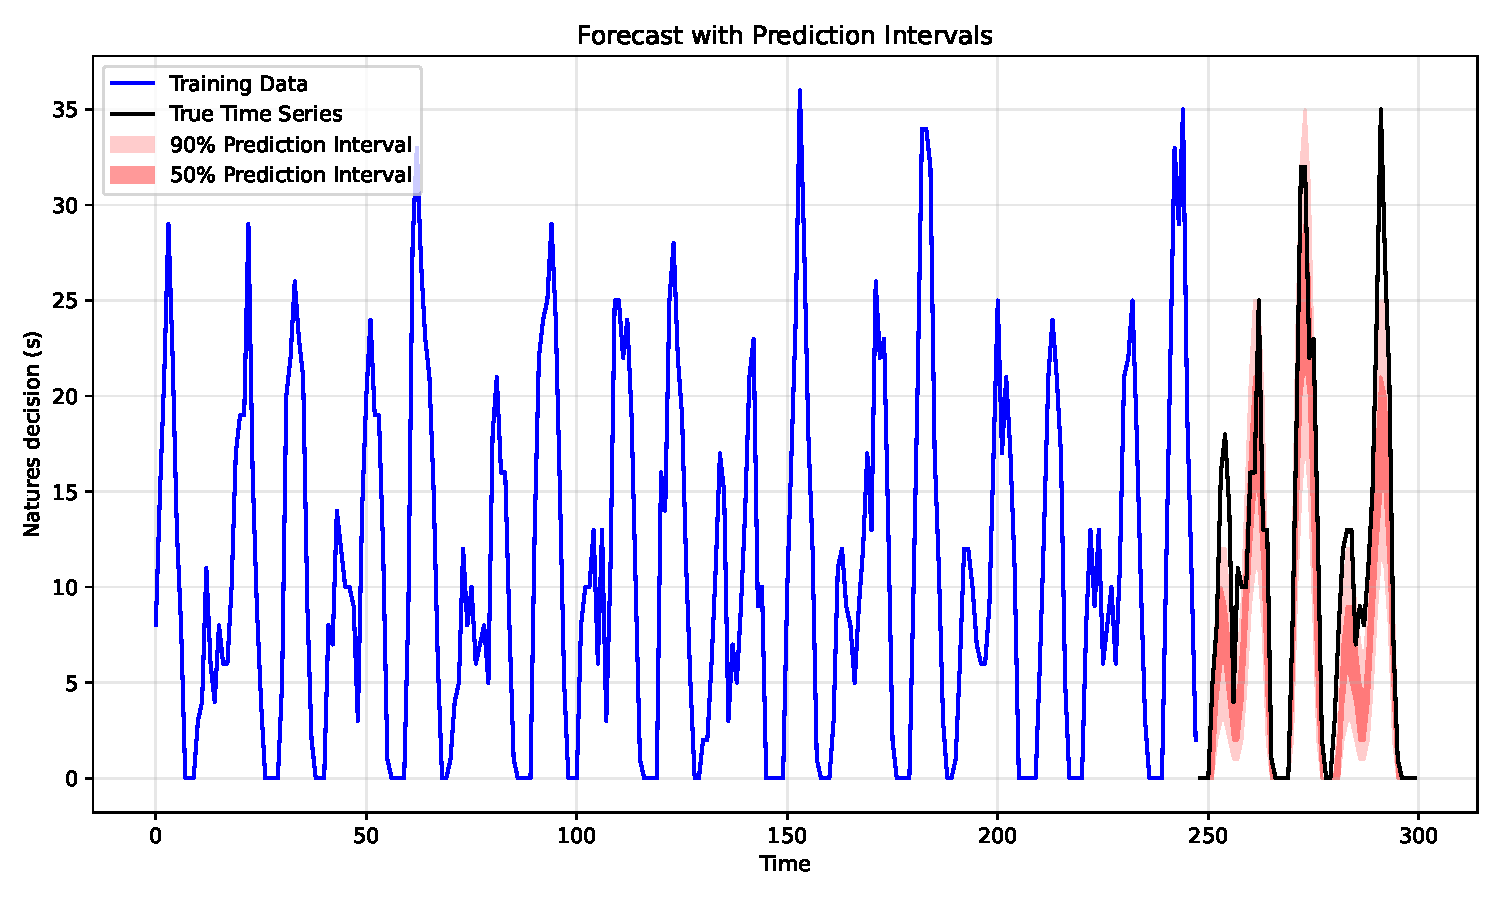
\includegraphics[width=1\textwidth]{figures/time_series.pdf}
	\caption{Natures decisions as a function of time. Blue denotes the historical data available for the Robot, red denote the forecast made by the Robot (based on the historical data) and the black denotes the true future values for reference (not used).}
	\label{fig:ts}
\end{figure}
\begin{definition}[Baseline Policy]  
	\label{def:baseline}
	The baseline policy is an $(R, Q)$ inventory policy~\citep{bartmann1992inventory,axsaeter2006inventory}, where the reorder point $R$ determines when to reorder, and the batch quantity, $Q$, is based on the expectation of Natures decisions
	\begin{equation}  
		\upsilon_t' = \max(\text{round}(\mathbb{E}[\zeta_t|D, I] + R - N_0), 0).  
	\end{equation}  
	The rounding ensures the order quantity is an integer, and the maximum function prevents negative orders.
\end{definition}

Given the above setup, figure \ref{fig:per} presents a heatmap illustrating the Policy Efficiency Ratio (PER) as a function of the reorder point $R$ and the cost-to-holding ratio $\frac{c}{h}$. From the figure, several patterns emerge. In general there seem to be bands of approximately constant PER following $R\sim \ln\frac{c}{h}$ -lines. This band represent the optimal balancing point for $R$ for a given $\frac{c}{h}$. At $\frac{c}{h}=1, R=0$ the PER achieves its maximum at $\simeq 1$, which makes intuitive sense since if $h=c$, the cost function is balanced and the optimal balancing point would be at $R=0$. The maximum value of the band slightly decrease for increasing $\frac{c}{h}$, with PER$\sim 0.9$ as a mean value. Hence, even in case where the reorder point $R$ is optimized perfectly, there is a significantly higher expected cost (around $10\%$) for the baseline (R,Q) - policy relative to the optimal policy (theorem \ref{theorem:opt_policy}). 
\begin{figure}[h!]
	\centering
	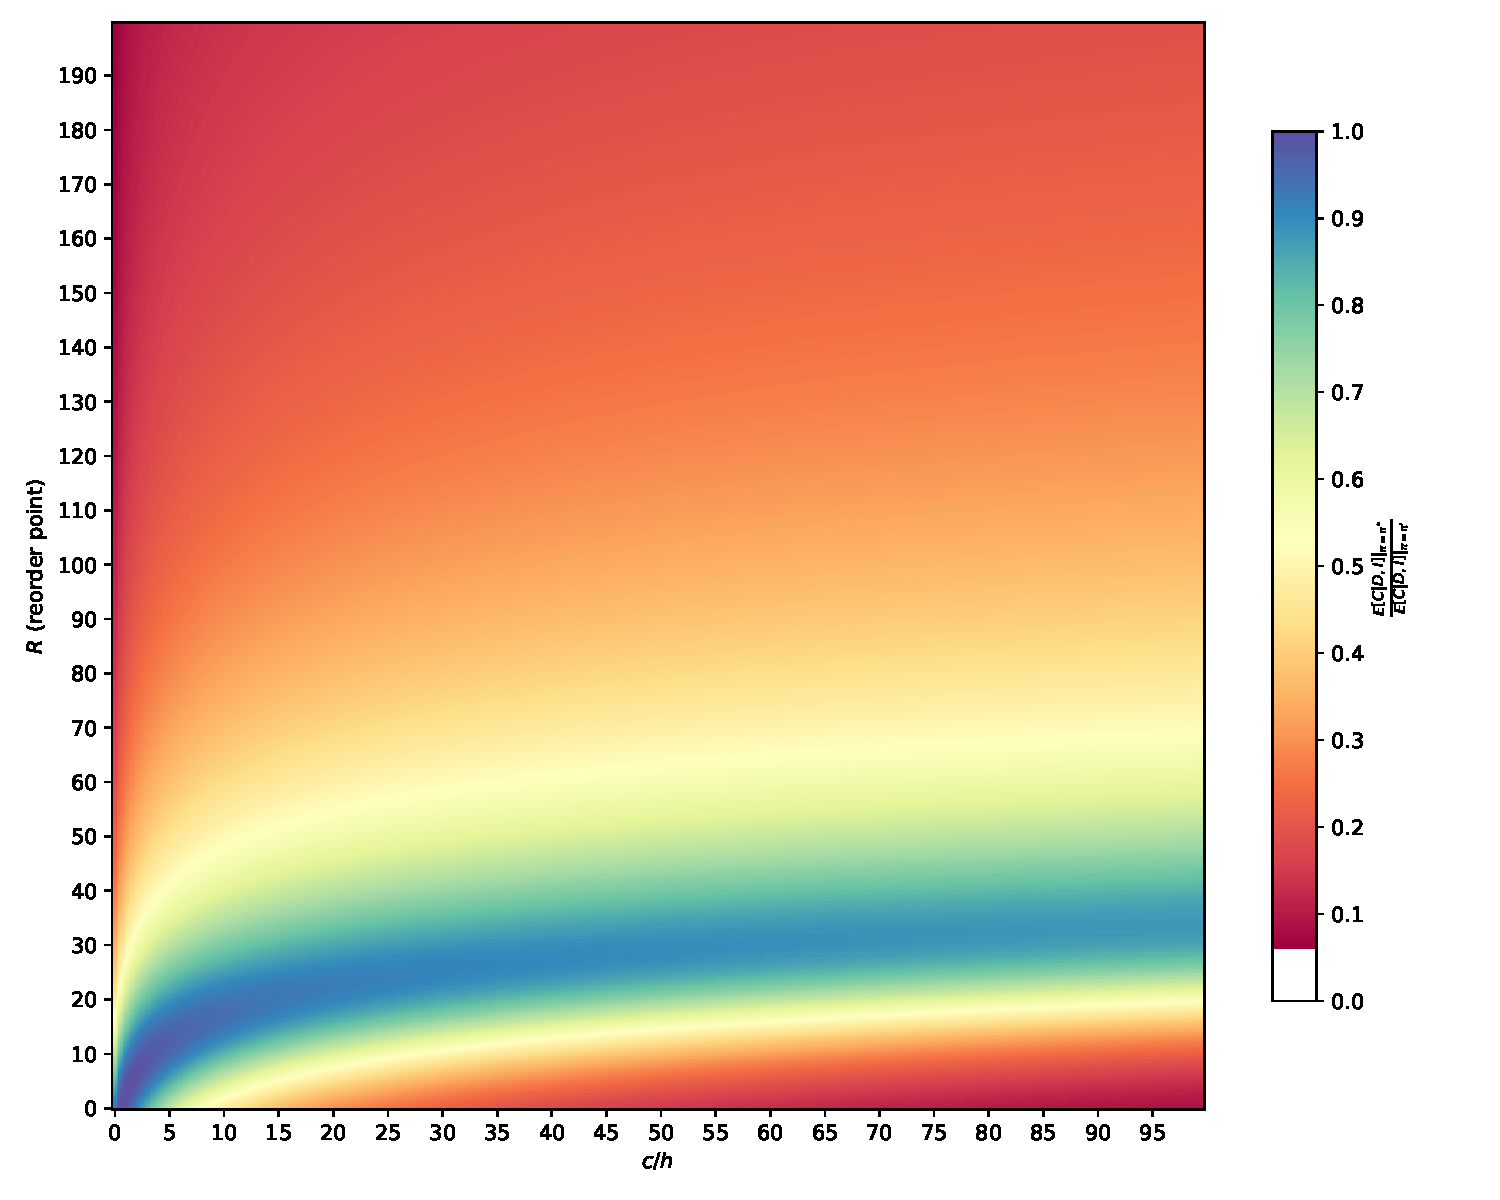
\includegraphics[width=1\textwidth]{figures/per.pdf}
	\caption{Heatmap of the policy efficiency ratio (PER) calculated using equations \eqref{eq:expected_cost}, \eqref{eq:per_def}, definition \ref{def:baseline} and theorem \ref{theorem:opt_policy} with $N_0=37$, $L=6$ and Natures decisions shown in figure \ref{fig:ts}.}
	\label{fig:per}
\end{figure}